\chapter{Task}
\label{ch:task}
Eventually, it is the generic ability to perform every conceivable task
that turns a computing device into a versatile universal tool. Consequently,
the issues of modeling and orchestrating of tasks are fundamental in the design of any OS.
Of course, we cannot expect a single fixed tasking metaphor to be the ideal solution
for all possible kinds of systems and modes of use. For example, different metaphors are
probably appropriate in the cases of a closed mainframe system serving a large set of users
in time-sharing mode, on one hand, and of a personal workstation operated by a single user
at a high degree of interactivity, on the other.

In the case of Oberon, we have consciously concentrated on the domain of personal workstations.
More precisely, we have directed Oberon's tasking facilities towards a single-user interactive
personal workstation that is possibly integrated into a local area network.

We start in \ref{sec:task} with a clarification of the technical notion of task.
In \ref{sec:scheduler} we continue with a detailed explanation of the scheduling strategy.
Then, in \ref{sec:command} we introduce the concept of command.
Finally, \ref{sec:toolbox} provides an overview of predefined system-oriented toolboxes,
i.e. coherent collections of commands devoted to some specific topic,
e.g. system control and diagnosis, display management, and file management.

\section{The Concept of Task}
\label{sec:task}
In principle, we distinguish 2 categories of tasks in Oberon:
\begin{table}[h!]
  \centering
  \begin{tabular}{r l}
    \small{INTERACTIVE}& bound to local regions on the display \\
                       & and interactions with their contents, \\
    \small{BACKGROUND} & system-wide and not necessarily related\\
                       & to any specific displayed entity.
  \end{tabular}
\end{table}

\subsection{Interactive Tasks}
Every interactive task is represented by a so-called viewer. Viewers constitute the interface
to Oberon's display-system. They embody a variety of roles that are collected in an abstract
data type \verb|Viewer|. We shall give a deeper insight into the display system in \ref{ch:display}.
For the moment it suffices to know that viewers are represented graphically as rectangles
on the display screen and that they are implicit carriers of interactive tasks.
Fig \ref{fig:dispcfg} shows a typical Oberon display screen that is divided up into 6
viewers corresponding to 6 simultaneously active interactive tasks.
\begin{figure}[h!]
  \centering
  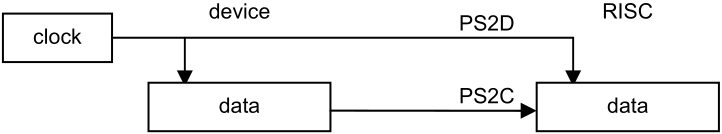
\includegraphics[width=.9\textwidth]{i/3.png}
  \caption{Typical display configuration with tool track on the right}
  \label{fig:dispcfg}
\end{figure}

In order to get firmer ground under our feet, we now present the programmed declaration
of type \verb|Viewer| in a slightly abstracted form:
\begin{verbatim}
  Viewer = POINTER TO ViewerDesc;
  ViewerDesc = RECORD X,Y,W,H, state: INT;
                      handle: Handler END;
\end{verbatim}
\verb|X|, \verb|Y|, \verb|W|, \verb|H| define the viewer's rectangle on the screen:
\begin{itemize}
  \item[] location \verb|X|, \verb|Y| of the lower left corner relative to the display origin,
  \item[] width \verb|W| and height \verb|H|.
\end{itemize}
\verb|state| informs about the current state of visibility
\begin{table}[h!]
  \centering
  \begin{tabular}{l}
    \verb|visible|, \\
    \verb|closed|, \\
    \verb|covered|
  \end{tabular}
\end{table}
\\while \verb|handle| represents the functional interface of viewers:
\begin{verbatim}
  Handler = PROC(V: Viewer; VAR M: ViewerMsg);
\end{verbatim}
where \verb|ViewerMsg| is some base type of messages
whose exact declaration is of minor importance for now:
\begin{verbatim}
  ViewerMsg = RECORD (*basic parameter fields*) END;
\end{verbatim}
However, we should point out the use of object-oriented (OO) terminology. It is justified because
\verb|handle| is a procedure variable (a handler) whose identity depends on the specific viewer.
A call \verb|V.handle(V, M)| can therefore be interpreted as the sending of a message \verb|M|
to be handled by the method of the receiving viewer \verb|V|.

We recognize an important difference between the standard OO model and our handler paradigm.
The standard model is closed in the sense that only a fixed set of messages is understood
by a given class of objects. In contrast, the handler paradigm is open because it defines
just the root (\verb|ViewerMsg|) of a potentially unlimited tree of extending message types.
For example, a concrete handler might be able to handle messages of type:
\begin{verbatim}
  MyViewerMsg = RECORD (ViewerMsg)
                  mypar: MyParameters
                END;
\end{verbatim}
which is an extended type of \verb|ViewerMsg|.

It is worth noting that our open OO model is extremely flexible. Notably, extending the set
of message types that are handled by an object is a mere implementation issue, that is, it
has no effect at all on the object’s compile-time interface and on the system integrity.
It is fair to mention though that such a high degree of extensibility does not come for free.
The price to pay is the obligation of explicit message dispatching at runtime.
The following chapters will capitalize on this property.

Coming back to the perspective of tasks, we note that each sending of a message to a viewer
corresponds to an activation or reactivation of the interactive task that it represents.

\subsection{Background Tasks}
Oberon background tasks are not connected a priori with any specific aggregate in the system.
Seen technically, they are instances of an abstract data type consisting of type declarations
\verb|Task| and \verb|TaskDesc| together with intrinsic operations \verb|NewTask|,
\verb|Install| and \verb|Remove|:
\begin{verbatim}
  Task = POINTER TO TaskDesc;
  TaskDesc = RECORD state: INT; handle: PROC END;
  PROC NewTask(h: PROC; period: INT): Task;
  PROC Install(T: Task);
  PROC Remove (T: Task);
\end{verbatim}
The procedures \verb|Install| and \verb|Remove| are called explicitly in order to transfer
the state of the specified task from \verb|offline| to \verb|idle| and from \verb|idle| to
\verb|offline| respectively. Installed tasks take their turns in becoming \verb|active|,
that is, in being executed. The installed handlers are simple, parameterless procedures
specifying their own actions and conditions for execution, with one exception:
Resumption may be delayed until a certain period of time has elapsed.
This period is specified in milliseconds when a task is created.

The following 2 examples of concrete background tasks may serve a better understanding of
our explanations. The 1st is a system-wide garbage collector collecting unused memory.
The 2nd is a network monitor accepting incoming data on a local area network. In both
examples the state of the task is captured entirely by global system variables. We shall
come back to these topics in \ref{ch:mm} and \ref{ch:net} respectively.

We should not end without drawing an important conclusion. Transfers of control between tasks
are implemented in Oberon as ordinary calls and ordinary procedures returns (procedure
variables, actually). Preemption is not possible. From that we conclude, active tasks periods
are sequentially ordered and controlled by a single thread. This simplification pays well:
Locks of common resources are completely dispensable and deadlocks are not a topic.

\section{The Task Scheduler}
\label{sec:scheduler}
We start from the general assumption that, at any given time, a number of well-determined
tasks are ready in the system to be serviced. Remember that 2 categories of tasks exist:
interactive and background ones. They differ substantially in the criteria of activation
or reactivation and in the priority of dispatching. Interactive tasks are (re)activated
exclusively upon interactions by the user and are dispatched with high priority.
In contrast, background tasks are polled with low priority.

We already know that interactive tasks are activated by sending messages. The types of messages
used for this purpose are \verb|InputMsg| and \verb|ControlMsg| reporting keyboard events
and mouse events respectively. Slightly simplified, they are declared as
\begin{verbatim}
  InputMsg = RECORD (ViewerMsg) id, X, Y: INT;
                      keys: SET; ch: CHAR END;

  ControlMsg = RECORD (ViewerMsg) id,X,Y: INT END;
\end{verbatim}
The field \verb|id| specifies the exact request transmitted with this specific reactivation.
In the case of \verb|InputMsg| the possible requests are consume (the character specified
by field \verb|ch|) and track (mouse, starting from state given by \verb|keys| and \verb|X|,
\verb|Y|). In case of \verb|ControlMsg| the choice is mark (the viewer at position \verb|X|,
\verb|Y|) or neutralize. Mark means moving the global system pointer (typically represented
as a star-shaped mark) to the current position of the mouse. Neutralizing a viewer
is equivalent to removing all marks and graphical attributes from this viewer.

All tasking facilities are collected in 1 module, called \verb|Oberon|. In particular, the
module's definition exposes the declarations of the abstract data type \verb|Task| and of
the message types \verb|InputMsg| and \verb|ControlMsg|. The module's most important
contribution, however, is the task scheduler (often referred to as “Oberon loop”)
that can be regarded as the system's dynamic center.

Before studying the scheduler in detail we need some more preparation. We start with the
institution of the focus viewer. By definition, this is a distinguished viewer that by
convention consumes subsequent keyboard input. Note that we identify the focus viewer with
the focus task, hereby making use of the one-to-one correspondence between viewers and tasks.

Module \verb|Oberon| provides the following facilities in connection with the focus viewer:
A global variable \verb|FocusViewer|, a procedure \verb|PassFocus| for transferring the role
of focus to a new viewer, and a defocus variant of \verb|ControlMsg| for notifying the old
focus viewer of such a transfer.

The implementation details of the abstract data type \verb|Task| are hidden from the clients.
It is sufficient to know that all task descriptors are organized in a ring and that a pointer
points to the previously activated task. The ring is guaranteed never to be empty because the
above mentioned garbage collector is installed as a permanent sentinel task at system loading time.

The following is a slightly abstracted version of the actual scheduler code operating on the
task ring. It should be associated with procedure \verb|Loop| in the module \verb|Oberon|.
\begin{verbatim}
  get mouse position and state of keys;
  REPEAT
    IF keyboard input available THEN read character
      IF character is escape THEN
        broadcast neutralize message to viewers
      ELSIF character is mark THEN
        send mark message to viewer containing mouse
      ELSE send consume message to focus viewer
      END;
      get mouse position and state of keys
    ELSIF at least one key pressed THEN
      REPEAT
        send track message to viewer containing mouse;
        get mouse position and state of keys
      UNTIL all keys released
    ELSE (*no key pressed*)
      send track message to viewer containing mouse;
      take next task in ring as current task;
      call its handler
              (if specified time period has elapsed)
      get mouse position and state of keys
    END 
  UNTIL FALSE
\end{verbatim}
The system executes a sequence of uninterrupted procedures (tasks). Interactive tasks are
triggered by input data being present, either from the keyboard, mouse, or other input sources.
Background tasks are taken up in a round-robin manner. Interactive tasks have priority.

Having consciously excluded exceptional program behavior in our explanations so far, some
comments about the way of runtime continuation in the case of a failing task or, in other
words, in the case of a trap are in order here. On the (abstract) level of tasks, we can
identify 3 sequential actions of recovery taken after a program failure:
\begin{verbatim}
  recovery after program failure =
    BEGIN save current system state;
      call installed trap handler;
      roll back to start of task scheduler
    END
\end{verbatim}
Essentially, the system state is determined by the values of all global and local variables
at a given time. The trap handler typically opens an extra viewer displaying the cause of
the trap and the saved system state. Notice in the program fragment above that background
tasks are removed from the ring after failing. This is an effective precaution against
cascades of repeated failures. Obviously, no such precaution is necessary in the case of
interactive tasks because their reactivation is under control of the user of the system.

Summarizing the essence of the Oberon tasking system:
\begin{itemize}
  \item A multitasking system based on a 2-category model
  \begin{description}
    \item[Interactive] interfacing with the display system,
      high-priority scheduled upon user interactions;
    \item[Background] stand-alone, low-priority scheduled.
  \end{description}
  \item Task activations are modeled as message passing,
    eventually, procedures calls assigned to variables.
    They're sequentially ordered, controlled by a single thread.
\end{itemize}

\section{The Concept of Command}
\label{sec:command}
An OS constitutes a general purpose platform on which applications can build upon. To
software designers the platform appears as interface to "the system" and (in particular)
to the underlying hardware. Unfortunately, interfaces defined by conventional OSes often
suffer from an all too primitive access mechanism that is based solely on the concept of
"software interrupt" or "supervisor call" and on files taking the role of “connecting pipes".
The situation is especially ironic when compared with the development of high-level
PLs towards extreme abstraction.

We have put greatest emphasis in Oberon on closing the semantic gap between applications
and the system platform. The result of our efforts is a highly expressive and consistent
\emph{application programming interface} (API) in the form of an explicit hierarchy of
module definitions. Perhaps the most significant and notable outcome of this approach is
a collection of very powerful and system-wide abstract data types such as \verb|Task|,
\verb|Frame|, \verb|Viewer|, \verb|File|, \verb|Font|, \verb|Text|, \verb|Module|,
\verb|Reader|, \verb|Scanner|, \verb|Writer|, etc.

\subsection{Atomic Actions}
The most important generic function of any OS is executing programs. A clarification of
the term program as it is used in Oberon comprises 2 views: a static and a dynamic one.
\begin{description}
  \item[Statically,] program means a software package with an \emph{entry point}.
More formally, it is a pair \verb|(M*, P)|, where \verb|M| is a module, \verb|P| is an
\emph{exported parameterless procedure} of \verb|M|, and \verb|M*| denotes the hierarchy
consisting of \verb|M| itself and all imported modules, directly or indirectly.

Note: 2 different hierarchies \verb|M*| and \verb|N*| are not generally disjoint, rather,
intersect a superset of the OS.

  \item[Dynamically viewed,] it is an \emph{atomic action} called \emph{command},
operating on the global system state. Here \emph{atomic} means \emph{no user interaction}.
This definition is just a necessary consequence of our \emph{non-preemptive task model}
scheduling with the benefit of a single \emph{carrier thread}. We can argue like this:

When a traditional interactive program requires input from the user, the current task is
normally preempted in favor of another task that produces the required input data. Therefore,
a traditional interactive program can be viewed as a sequence of atomic actions interrupted
by actions that possibly belong to other programs. Whereas interruption in traditional systems
may occur at any time, yet in Oberon it can occur only after task (command) completion.
\end{description}

Quintessentially, programs are represented as commands: exported parameterless procedures
not interacting with the user.

Returning to programs calling and execution we now arrive at the following refined version:
\begin{verbatim}
  call program(M*, P) = BEGIN
    load module hierarchy M*;
    call command P
  END
\end{verbatim}
The system interface to the command mechanism itself is again provided by \verb|Oberon|.
Its primary operation is to "call command by name and pass actual parameters":
\begin{verbatim}
  PROC Call(name: ARRAY OF CHAR;
            pars: ParList; VAR res: INT);
\end{verbatim}
\begin{table}[h!]
  \centering
  \begin{tabular}{r l}
  \verb|name| & the desired command name in form of \verb|M.P|, \\
  \verb|pars| & the actual parameters list (APL), and \\
  \verb|res|  & the result code.
  \end{tabular}
\end{table}

But in fact we have separated the setting of parameters:
\begin{verbatim}
  PROC SetPar(F: Display.Frame;
              T: Texts.Text; pos: INT);
\end{verbatim}
\begin{table}[h!]
  \centering
  \begin{tabular}{r l}
                \verb|F| & indicates the calling viewer, \\
    Pair \verb|(T, pos)| & specifies the starting position of a text.
  \end{tabular}
\end{table}

from the actual call:
\begin{verbatim}
  PROC Call(name: ARRAY OF CHAR; VAR res: INT);
\end{verbatim}

Notice the occurrence of yet another abstract data type \verb|Text|, exported by \verb|Texts|.
We shall devote \ref{ch:text} to a thorough discussion of Oberon's text system.
For the moment we can simply look at a text as a sequence of characters.

The APL is handed over to the command by \verb|Oberon| as an exported global variable:
\begin{verbatim}
  Par: RECORD vwr: Viewers.Viewer;
         frame: Display.Frame;
         text: Texts.Text; pos: INT
       END
\end{verbatim}
In principle, commands operate on the entire system and can access the current global state
via the system's powerful abstract modular interface, of which the APL is just one component.
Another one is the so-called \emph{system log} which is a system-wide protocol reporting on
the progress of command execution and on exceptional events in chronological order. The log
is represented as a global variable:
\begin{verbatim}
  Log: Texts.Text;
\end{verbatim}
It should have become clear by now that implementers of commands may rely on a rich arsenal
of abstract global facilities that reflect the current system state and make it accessible.
In other words, they may rely on a high degree of system integration. Therefore, Oberon
features an extraordinarily broad spectrum of mutually integrated facilities. For example,
the system distinguishes itself by a complete integration of the abstract data types
\verb|Viewer| (\ref{ch:display}) and \verb|Text| (\ref{ch:text}) that we encountered above.

\verb|Oberon| assists the integration of these types with the following conceptual features,
including the 1st 2 we have just introduced:
\begin{enumerate}
  \item Standard parameter list for commands,
  \item system log,
  \item generic text selection, and
  \item generic copy viewer.
\end{enumerate}
At this point we should add a word of clarification to our use of the term \emph{generic}.
It is synonymous with "interpretable individually by any viewer (interactive task)" and is
typically used in connection with messages or orders whose receiver's exact identity is unknown.

Let us now go into a brief discussion of the generic facilities
without, however, leaving the level of our current abstraction and understanding.

\subsection{Generic Text Selection}
Textual selections are characterized by
\begin{table}[h!]
  \centering
  \begin{tabular}{l}
    a text, \\
    a stretch of characters within that text, and \\
    a time stamp.
  \end{tabular}
\end{table}

Without further qualification "the text selection" always means "the most recent text selection".
It can be obtained programmatically by calling:
\begin{verbatim}
  PROC GetSelection(VAR text: Texts.Text;
                    VAR beg, end, time: LONGINT);
\end{verbatim}
The parameters specify the desired stretch of text starting at position \verb|beg| and ending
at \verb|end-1| as well as the associated time stamp. The procedure is implemented in form of
a broadcast of a socalled selection message to all viewers. The declaration of this message is
\begin{verbatim}
  SelectionMsg = RECORD (ViewerMsg) text: Texts.Text;
                          beg, end, time: INT  END;
\end{verbatim}

\subsection{Generic Copy Viewer}
Generic copying is synonymous with reproducing and cloning. It is the most elementary
generic operation possible. Again, a variant of type \verb|ViewerMsg| is used
for the purpose of transmitting requests of the desired type:
\begin{verbatim}
  CopyMsg = RECORD (ViewerMsg) vwr:Viewers.Viewer END;
\end{verbatim}
Receivers of a copy message typically generate a clone of themselves
and return it to the sender via field \verb|vwr|.

Let us now summarize the concept of command in Oberon:
\begin{itemize}
  \item As an OS Oberon presents to clients a highly expressive \emph{modular interface}
    that exports many powerful abstract data types like \verb|Viewer| and \verb|Text|.
    A rich arsenal of global data types and generic facilities achieve
    \emph{system integration} at a high degree.
  \item Programs are modeled as \emph{commands},
    \emph{exported parameterless procedures} not interacting with the user.
  \item The collection of commands provided by a module appears as its \emph{user interface}.
    Parameters are passed to commands via a global parameter list,
    registered by the calling task in the central \verb|Oberon|.
  \item Commands operate on the global state of the system.
\end{itemize}

\section{Toolboxes}
\label{sec:toolbox}
Modules typically appear in 3 different forms.
\begin{itemize}
  \item[$1^{st}$] encapsulates some data, which can be accessed only through exported
    procedures and functions. \verb|FileDir|, encapsulating the file directory and
    protecting it from disruptive access, is a good example.
  \item[$2^{nd}$] represent an abstract data type, exporting it and its associated operators.
    \verb|Files|, \verb|Modules|, \verb|Viewers|, and \verb|Texts| are typical examples.
  \item[$3^{rd}$] collection of procedures pertaining to the same topic,
    like \verb|RS232| handling communication over a serial line.
\end{itemize}
Oberon adds a $4^{th}$ form:
\begin{description}
  \item[\emph{toolbox}] A pure collection of commands on the \emph{top} of the modular hierarchy.
    Toolbox modules are "imported" by system users at run-time. In other words, their definitions
    define the user interface. Typical examples are \verb|System| and \verb|Edit|.
\end{description}
As a rule of thumb there exists a toolbox for every topic or application.
As an example of a toolbox definition we quote an annotated version of \verb|System|:
\begin{verbatim}
  DEFINITION System;
    (*System management, Ch. 3 and 8*)
    PROC SetUser;  (*identification*)
    PROC SetFont;  (*for typed text*)
    PROC SetColor; (*for typed text&graphics*)
    PROC SetOffset;(*for typed text*)
    PROC Date;     (*set/get date&time*)
    PROC Collect;  (*garbage*)
    (*Display management, Ch. 4*)
    PROC Open;  (*viewer*)
    PROC Close; (*viewer*)
    PROC CloseTrack;
    PROC Recall;(*most recently closed viewer*)
    PROC Copy;  (*viewer*)
    PROC Grow;  (*viewer*)
    PROC Clear; (*log*)
    (*Module management, Ch. 6*)
    PROC Free;        (*specified modules*)
    PROC ShowCommands;(*of specified module*)
    PROC ShowModules; (*show loaded modules*)
    (*File management, Ch. 7*)
    PROC Directory;
    PROC CopyFiles;
    PROC RenameFiles;
    PROC DeleteFiles;
    (*System inspection, Ch. 8*)
    PROC Watch;(*tasks, memory&disk storage*)
  END System;
\end{verbatim}
An important consequence of our integrated systems approach is the possibility of constructing
a universal, interactive command interpreter bound to viewers of textual contents. If the text
obeys the following syntax (specified in EBNF), we call it command tool:
\begin{verbatim}
  CommandTool = {[Comment]CommandName[ParameterList]}
\end{verbatim}
If present, the parameter list is made available to the called command via fields \verb|text|
and \verb|pos| in the global variable \verb|Par| that is exported from \verb|Oberon|. Because
this parameter list is interpreted individually by each command, its format is completely open.
However, we postulate some conventions and rules for the purpose of a standardized user interface:
\begin{enumerate}
  \item The elements of a textual parameter list (TPL) are universal syntactical tokens
    like name, literal string, integer, real number, and special character.
  \item An arrow "\^{}" in the TPL refers to the current text selection for continuation.
    In the special case of the arrow following the command name immediately,
    the entire parameter list is represented by the text selection.
  \item An asterisk "*" in the TPL refers to the currently marked viewer.
    Typically, the asterisk replaces the name of a file.
    In such a case the contents of the viewer marked by the system pointer (star)
    is processed by the command interpreter instead of the contents of a file.
  \item An at-character "@" in the TPL indicates that the selection
    marks the (beginning of the) text which is taken as operand.
  \item A terminator-character "\~{}" terminates the TPL in case of a variable number of parameters.
\end{enumerate}

Because command tools are ordinary, editable texts (in contrast to menus in conventional systems),
they can be customized "on the fly", which makes the system highly flexible.
We refer again to Fig \ref{fig:dispcfg} that shows a typical Oberon screen layout consisting
of 2 vertical tracks,
\begin{enumerate}
  \item a wider user track on the left, and\\
  \textcolor{gray}{3 documents are displayed in the user track:}
  \begin{enumerate}
    \item a text,
    \item a graphic, and
    \item a picture.
  \end{enumerate}
  \item a narrow system track on the right,\\
  \textcolor{gray}{where we find 1 logviewer displaying the system log, 2 tool-viewers making available}
  \begin{enumerate}
    \item the standard system tool, and
    \item a customized private tool respectively.
  \end{enumerate}
\end{enumerate}

In concluding this chapter, let us exemplify the concepts of command and tool by the system
control section of the \verb|System| toolbox. Consisting of the commands
\begin{table}[h!]
  \centering
  \begin{tabular}{r l}
    \verb|SetUser|  & \small{installing the user's identification,}\\
    \verb|Date|     & \small{displaying or setting the system date and time,}\\
    \verb|SetFont|  & \small{presetting the system type-font for typed text,}\\
    \verb|SetColor| & \small{setting the system color, and}\\
    \verb|Collect|  & \small{activating the garbage collector.}
  \end{tabular}
\end{table}
\\They are used to control system-wide facilities (detail each).

In summary,
\begin{itemize}
  \item[-] a toolbox is a special module, defined as a \emph{collection of commands};
  \item[-] appearing at the top of the modular hierarchy, the entire toolboxes
    fix the \emph{user interface} for the system;
  \item[-] command tools are sequences of textually represented command calls,
    editable and customizable;
  \item[-] in a typical screen layout, tools are displayed in the viewers
    within the \emph{system track}.
\end{itemize}
